\documentclass[11pt, A4]{article}
\usepackage[utf8]{inputenc}
\usepackage{amsfonts}
\usepackage{tikz}
\usetikzlibrary{automata, positioning, arrows}
\setlength{\parindent}{0em}
\setlength{\parskip}{1em}

\title{Test Tikz}

\begin{document}

\begin{titlepage}
  \maketitle
\end{titlepage}

\section{Example tikz state machines}

\begin{figure}[ht]
  \centering
  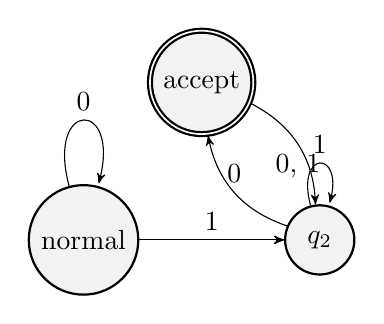
\begin{tikzpicture}
    % settings can be global or per picture
    \tikzset{
      ->,
      >=stealth',
      node distance=3cm,
      every state/.style={thick, fill=gray!10},
      initial text=$ $,
    }

    % states
    \node[state] (q1) {normal};
    \node[state, initial, right of=q1] (q2) {$q_2$};
    \node[state, accepting] at (1.5, 2) (q3) {accept};

    % transitions
    \draw (q1) edge[loop above] node{0} (q1)
          (q1) edge[above] node{1} (q2)
          (q2) edge[loop above] node{1} (q2)
          (q2) edge[bend left, above] node{0} (q3)
          (q3) edge[bend left, below] node{0, 1} (q2);

  \end{tikzpicture}
  \caption{Example}
  \label{fig:example1}
\end{figure}

\begin{figure}[ht]
  \centering
  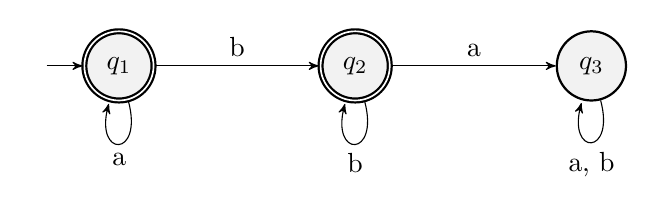
\begin{tikzpicture}
    % settings can be global or per picture
    \tikzset{
      ->,
      >=stealth',
      node distance=3cm,
      every state/.style={thick, fill=gray!10},
      initial text=$ $,
    }

    % states
    \node[state, accepting, initial] (q1) {$q_1$};
    \node[state, accepting, right of=q1] (q2) {$q_2$};
    \node[state, right of=q2] (q3) {$q_3$};

    % transitions
    \draw (q1) edge[loop below] node{a} (q1)
          (q1) edge[above] node{b} (q2)
          (q2) edge[loop below] node{b} (q2)
          (q2) edge[above] node{a} (q3)
          (q3) edge[loop below] node{a, b} (q3);

  \end{tikzpicture}
  \caption{FSM for $\{a^nb^m | n\geq0, m\geq0\}$}
  \label{fig:example2}
\end{figure}

Hello \ref{fig:example2}.

\begin{figure}[ht]
  \centering
  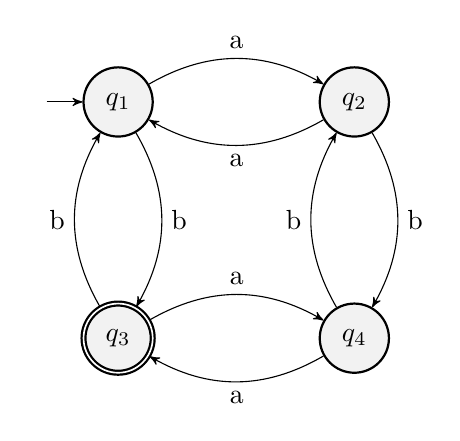
\begin{tikzpicture}
    % settings can be global or per picture
    \tikzset{
      ->,
      >=stealth',
      node distance=3cm,
      every state/.style={thick, fill=gray!10},
      initial text=$ $,
    }

    % states
    \node[state, initial] (q1) {$q_1$};
    \node[state, right of=q1] (q2) {$q_2$};
    \node[state, accepting, below of=q1] (q3) {$q_3$};
    \node[state, right of=q3] (q4) {$q_4$};

    % transitions
    \draw (q1) edge[bend left, above] node{a} (q2)
          (q2) edge[bend left, below] node{a} (q1)
          (q1) edge[bend left, right] node{b} (q3)
          (q3) edge[bend left, left] node{b} (q1)
          (q3) edge[bend left, above] node{a} (q4)
          (q4) edge[bend left, below] node{a} (q3)
          (q2) edge[bend left, right] node{b} (q4)
          (q4) edge[bend left, left] node{b} (q2);

  \end{tikzpicture}
  \caption{FSM for $\{w | w \quad \mathrm{has \quad even} \quad a\mathrm{'s
           \quad and \quad odd } \quad b\mathrm{'s}\}$}
  \label{fig:example3}
\end{figure}

\newpage
\section{Finite Automata}
A finite automata is a 5-tuple
$ (Q, \Sigma, \delta, s_0, F) $
where $Q$ is a finite set of states, $\Sigma$ is the input alphabet, $\delta$ is the
transition function, $s_0 \in Q$ is the start state, $F \subseteq Q$ is the set of accept states.

\begin{figure}[ht]
  \centering
  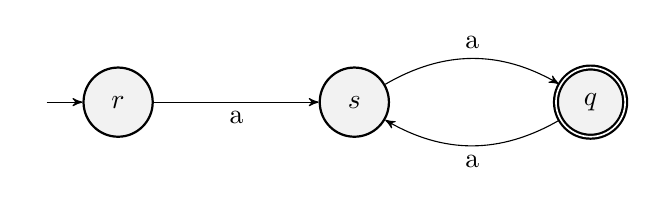
\begin{tikzpicture}
    % settings can be global or per picture
    \tikzset{
      ->,
      >=stealth',
      node distance=3cm,
      every state/.style={thick, fill=gray!10},
      initial text=$ $,
    }

    % states
    \node[state, initial] (r) {$r$};
    \node[state, right of=r] (s) {$s$};
    \node[state, accepting, right of=s] (q) {$q$};

    % transitions
    \draw (r) edge[below] node{a} (s)
          (s) edge[bend left, above] node{a} (q)
          (q) edge[bend left, below] node{a} (s);

  \end{tikzpicture}
  \caption{FSM for $\{a^n | n=2m, m>0, m \in \mathbb{N} \}$}
  \label{fig:example4}
\end{figure}


For the FSM in \emph{Figure \ref{fig:example4}}:
\begin{itemize}
  \item $Q = \{r, s, q\}$
  \item $\Sigma = \{a\}$
  \item $\delta : Q \times \Sigma \to Q$
  \item $s_0 = r$
  \item $F = \{q\}$
\end{itemize}

The combination of a state and a string is a configuration.
A configuration is a pair: $(q, w) \in Q \times \Sigma\ast, (q \in Q, w \in
\Sigma\ast)$.
With an original string of $aaaa$ the list of configurations for the FSM in
\emph{Figure \ref{fig:example4}} is:

\begin{itemize}
  \item $(r, aaaa)$
  \item $(s, aaa)$
  \item $(q, aa)$
  \item $(s, a)$
  \item $(q, \varepsilon)$
\end{itemize}

Let $(q, w)$ and $(q', w')$ be configurations, where:
$$w = aw'$$
for some letter $a \in \Sigma$, and
$$\delta(q, a) = q'$$
Then we say that $(q, w)$ yields $(q', w')$ in one step.

Therefore, $(q, aa)$ yields $(s, a)$ in one step in the example in \emph{Figure
\ref{fig:example4}}.

For configurations $(q, w)$ and $(q', w')$ we say that $(q, w)$ yields $(q', w'$
if there is a finite sequence of configurations
$$(q_1, w_1), (q_2, w_2), ..., (q_k, w_k)$$
Such that $(q_1, w_1)=(q,w), (q_k, w_k)=(q',w')$, and
$(q_i, w_i)$ yields $(q_{i+1}, w_{i+1})$ in one step for all $i=1, 2, ..., k-1$

The sequence of configurations defined above is called a \textbf{computation}

The finite automaton $M=(Q, \Sigma, \delta, s_0, F)$ \textbf{accepts} the string
$w \in \Sigma\ast$ if $(s_0, w)$ yields $(q, \varepsilon)$ where $q \in F$.

We say that the finite automaton $M$ \textbf{recognises} the language $A$ if
$A=\{w|M \quad \mathrm{accepts} \quad w\}$.

The language \textbf{recognised by} a finite automaton $M$ is denoted $L(M)$.

The language $A$ is called regular if there exists some finite automaton $M$
such that $A = L(M)$. (i.e. a finite automaton exists that recognises it)
\end{document}
